\begin{figure*}
\center{
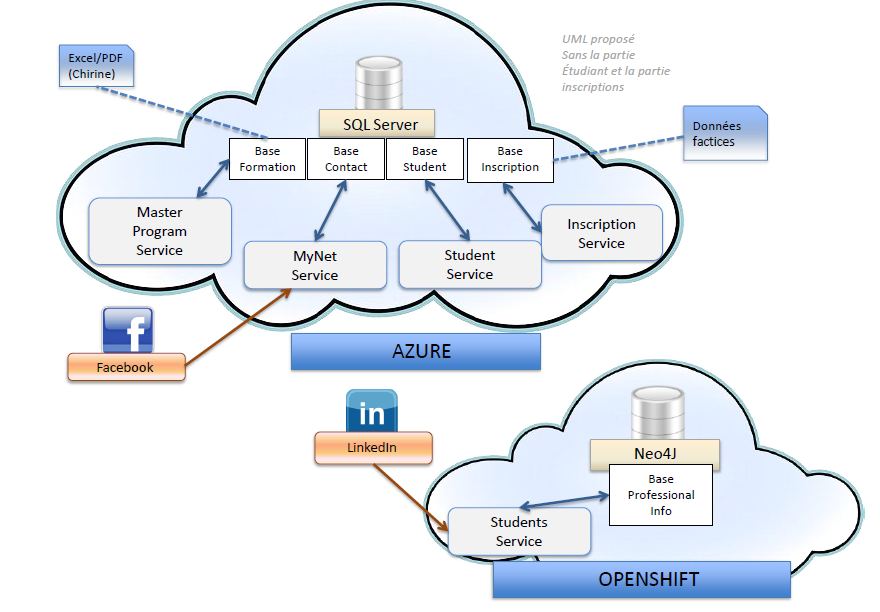
\includegraphics[width=0.60\textwidth]{use-case.png}
\caption{General distributed data storage service.\label{fig:storage}}}
\end{figure*}

According to our example scenario, we conducted an experience for implementing our data integration approach on a multi-cloud environment. We focussed on the implementation of a data as a service layer that integrates content from different services related to education but also related on data producers and consumers. Figure \ref{fig:storage} shows the general architecture of our scenario, deployed on Window Azure data store services and on Jelastic (https://jelastic.com), an open free cloud provider where we installed NE4J and Mongo NoSQL stores. The multi-cloud data as a service layer is a data provision platform storing clean data sets stemming from public data services (Linked in, Twitter, Facebook) accessible on Internet and also from private ones. 

The DaaS platform interacts recurrently with services in order to retrieve data and build collections that can be accessed by consumers. Each data service is characterized by the quality of data it provides, its availability and also by privacy and data ownership contrats provided as SLA contracts and enforced by security protocols. In the case of our MOOC scenario data concern public professional information about the users of our MOOC exported by Linked in. Such information and particularly their expertise supported by other contacts are used in order to determine the quality of the content they provide. Content and professional information are stored in data store deployed in Jelastic.  Our NoSQL support is configured for ensuring data availability and good data processing performance, given that our content is heterogeneous and it can be "critical" in our MOOC. Indeed, consumers can specify time delivery constraints that must be respected by our DaaS layer. Data concerning private data about users of our MOOC are stored in SQL Server on Azure. They are maintained according the  SLA contract provided for the less costly subscription to Azure, that corresponds to an education grant licence. We decided to manage information about courses programs in SQL Server since it seems that the relational model is well adapted for these type of data. Given the conditions of our subscription, and that the storage space to which we have access to Azure we decided to store the less voluminous data collections on this cloud. Data collections are services that have associated CRUD front-ends implemented using the Spring Roo library. Thus, data collections can be accessed by applications through their API our through an application. 

We proposed a global service that gives access to these databases in an integrated way, and can receive queries using a pivot language, UNQL in our case. The global service implements a  process for dealing with SLA and  the  query rewriting process. Global queries are expressed in UNQL and expected SLA in documents containing constraint expression are un-equalities as shown previously. For the time being our experiment does not deales with SLA derivation for choosing data services. SLA measures concern the delay in which results are delivered, the size of results, and the period in which queries are re-executed in order to get new or fresh data.
